\documentclass{article} % For LaTeX2e
\usepackage{nips15submit_e,times}
\usepackage{hyperref}
\usepackage{url}
%\documentstyle[nips14submit_09,times,art10]{article} % For LaTeX 2.09

\usepackage{listings}
\usepackage{graphicx}
\title{Weekly Report(July.8.2019-July.14.2019)}


% The \author macro works with any number of authors. There are two commands
% used to separate the names and addresses of multiple authors: \And and \AND.
%
% Using \And between authors leaves it to \LaTeX{} to determine where to break
% the lines. Using \AND forces a linebreak at that point. So, if \LaTeX{}
% puts 3 of 4 authors names on the first line, and the last on the second
% line, try using \AND instead of \And before the third author name.

\newcommand{\fix}{\marginpar{FIX}}
\newcommand{\new}{\marginpar{NEW}}

%\nipsfinalcopy % Uncomment for camera-ready version

\begin{document}


\maketitle

\begin{abstract}
This week I learned to use tensorbardX and continued to train AlexNet.
  
\end{abstract}

\section{Lessions from last week's questions}

\begin{itemize}
\item First, training data is more important than a network. We should always rebuild the network structure instead of resizing the input data.

\item Then I'd like to show my flowchart here. I am sorry to forget it last week. 

\begin{figure}[hb]
	\centering  %插入的图片居中表示
	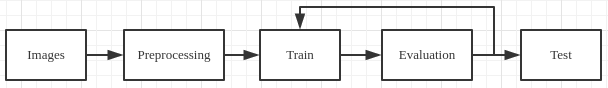
\includegraphics[width=0.4\textwidth]{6.png} 
	\caption{System Flow Chart}  %图片的名称
	\label{fig:f1}   %标签,用作引用
\end{figure}

\end{itemize}

\section{TensorBoardX}
With my buddy's suggestion, I use TensorBoardX to record my training result this time.

Store the result like this:
\begin{lstlisting}[language=python]
		from tensorboardX import SummaryWriter 
		writer = SummaryWriter(comment="train")
		writer.add_scalar('train', loss.item(), t)
\end{lstlisting}

And run it to show them by this:
\begin{lstlisting}[language=bash]
		tensorboard --logdir runs/
\end{lstlisting}

\begin{figure}[h]
	\centering  %插入的图片居中表示
	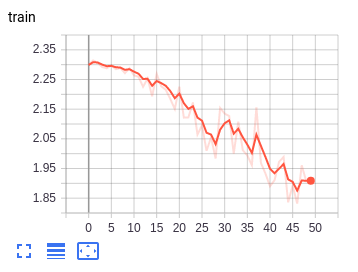
\includegraphics[width=0.4\textwidth]{1.png} 
	\caption{First loss line}  %图片的名称
	\label{fig:f1}   %标签,用作引用
\end{figure}

\section{AlexNet}
I rebuilt the structure of AlexNet. It didn't take me too much time so I spend more time to train and try to get some expected result. 

Figure 2 shows the new network. Combined to the origin one, I just changed some parameters, for example like kernel size, to adapt to input dataset and add Batch Normalization to avoid saturation.

\begin{figure}[ht]
	\centering  %插入的图片居中表示
	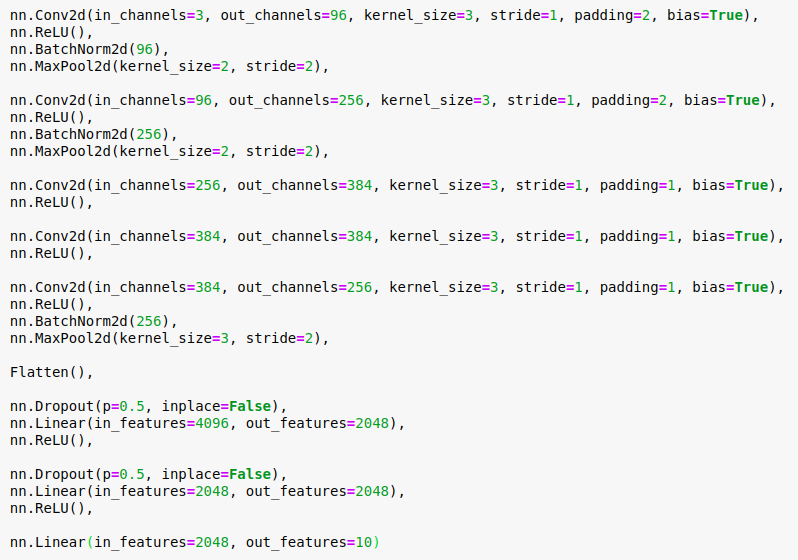
\includegraphics[width=0.8\textwidth]{2.png} 
	\caption{AlexNet Structure}  %图片的名称
	\label{fig:f1}   %标签,用作引用
\end{figure}

The visualization of the training process is in Figure 3. Definitely tensorboardX makes it more evident to know how the training works.

\begin{figure}[h]
	\centering  %插入的图片居中表示
	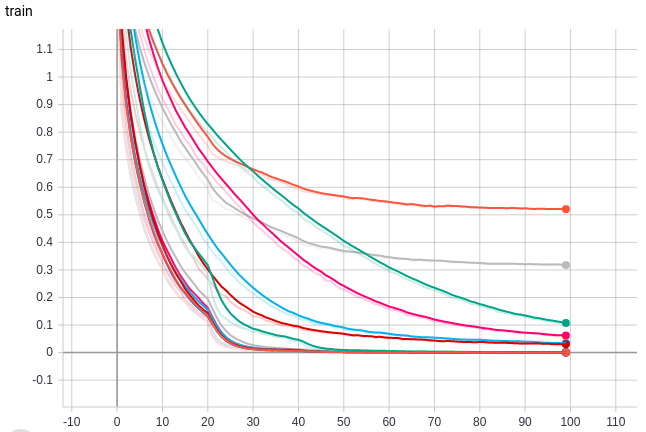
\includegraphics[width=0.8\textwidth]{5.png} 
	\caption{AlexNet Structure}  %图片的名称
	\label{fig:f1}   %标签,用作引用
\end{figure}

I trained different models with different hyper parameters and different optimizers. The real output is too much, I will just show some simple data here.

\begin{itemize}
\item The hyper parameters and their result of different models are showed below. Since it's the beginning, I set the learning rate start from 0.01 and multiple 1/3 for every 20 epoches.

\begin{table}[h]
\caption{learning\_rate=0.01, and multiples 1/3 for every 20 epoches}
%\label{sample-table}
\begin{center}
\begin{tabular}{c|c|c}
\multicolumn{1}{c}{\bf Batch Size} &\multicolumn{1}{c}{\bf Momentum} &\multicolumn{1}{c}{\bf Accuracy}
\\ \hline \\
64 & 0.9 & 87.59\% \\
64 & 0.95 & 88.08\%\\
128 & 0.9 & 88.09\%\\
128 & 0.95 & 87.56\%\\
\end{tabular}
\end{center}
\end{table}

\item I wonder whether learning rate is the critical factor making accuracy so high. So I keep it the same. The result is in table2. It seems that I am wrong.

\begin{table}[h]
\caption{learning\_rate=0.01, momentum=0.95}
%\label{sample-table}
\begin{center}
\begin{tabular}{c|c|c}
\multicolumn{1}{c}{\bf Batch Size} &\multicolumn{1}{c}{\bf Accuracy}
\\ \hline \\
64 & 87.44\% \\
128 & 87.61\% \\
256 & 87.27\% \\
\end{tabular}
\end{center}
\end{table}

\item I still tried another optimizer--Adadelta. Since Adadelta is said to train the network faster and more precisely. The Hype parameters and results are in table3. It seems not so good. In my opinion, learning rate may be a important factor. I will show it in next report.

\begin{table}[h]
\caption{learning\_rate=0.01, optimizer=Adadelta}
%\label{sample-table}
\begin{center}
\begin{tabular}{c|c|c}
\multicolumn{1}{c}{\bf Batch Size} &\multicolumn{1}{c}{\bf Accuracy}
\\ \hline \\
128 & 74.66\% \\
256 & 72.63\% \\
\end{tabular}
\end{center}
\end{table}

\end{itemize}

\section{Plan}
\begin{itemize}
\item Just as I said in the last report, I will start to use pre-trained VGG to build model and fine tune the model with cifar10. Time is limited, I will do as more as possible.
\end{itemize}
\end{document}
